%você pode organizar melhor suas imagens se criar subpastas nos chapters
\begin{figure}[ht!]
\centering

\caption{\textmd{Texto Texto Texto Texto Texto Texto Texto Texto Texto Texto Texto Texto Texto Texto Texto Texto Texto Texto Texto Texto Texto Texto Texto Texto Texto Texto Texto Texto}}
\label{fig:figuraex}
\fcolorbox{gray}{white}{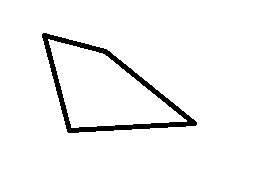
\includegraphics[width=0.5\textwidth]{images/captitulo1/figuraex.png}}

\fonteref{\citeauthor{manualufpe2020} (\citeyear{manualufpe2020})}
\end{figure}